\chapter{\xlabel{dimm}The Dynamic Iterative Map-Maker Explained}
\label{sec:dimm}

The Dynamic Iterative Map-Maker, hereafter just referred to as the
map-maker is the tool you will use to produce SCUBA-2 maps. It performs
all pre-processing steps to clean the data, followed by solving for
multiple signal components using an iterative algorithm, and regridding
the resulting time-series data to produce a final science map.

This chapter describes how the map-maker produces a science image
from raw SCUBA-2 data. It should be considered essential reading as it
provides an understanding of how your reduced image was produced. This is
particularly true if you wish to modify the default map-maker parameters.
\color{red}\textbf{ If you prefer to jump straight in to the data reduction go
to \cref{Chapter}{sec:pipe}{The SCUBA-2 Pipeline}.}\color{black}


\section{\xlabel{dimm_theory}How it works}

The map-maker works by producing individual models of the various
components that make up the signal recorded by each bolometer, one of
which is the required astronomical signal.  It models and removes each of
these components in order of decreasing magnitude, ultimately leaving
just the astronomical signal plus residual noise.  The modelled
components are listed in \cref{Table}{tab:mods}{tabulated} and described
more fully in \cref{Section}{sec:models}{The individual models}.

\textbf{The map-maker requires a configuration file to accompany each
reduction.} This file controls all aspects of the map-maker, including
details of the the pre-processing steps, which model components to include,
parameters that control the determination of each model, and the stopping
(or convergence) criteria.  There is a single generic default configuration
file called \file{dimmconfig.lis}.  Its configuration parameters are tabulated
in \cref{Appendix}{app:dimm}{an appendix}.

Often, the default configuration file will not give optimal results
for your particular observation. For this reason, specialised
configuration files have been developed which are tailored to
different science goals, be they detecting faint galaxies or mapping
large molecular clouds. A description of these specialised
configuration files can be found \cref{in Section}{sec:config}{here}
with listings \cref{in Appendix}{app:special}{this appendix}.


\section{The reduction step-by-step}

This section describes the basic map-making process used by the
default configuration.  It may be modified in many ways by suitable
changes to the parameter values in the configuration file.

\cref{Figure}{fig:dimm}{The graphic below} shows the flow chart of the
basic map-making process. It is divided into two sections: the pre-processing
stage where the data are cleaned, then the iterative stage where the different
models are subtracted, a sky map created and the convergence checked.


\begin{enumdesc}
\item[Initial cleaning and downsampling]
  The separate raw data files are first concatenated into a single time
  series for each sub-array (if possible --- see \latexhtml{the description
  of \emph{Data Chunking} on Page~\pageref{box:chunk})~}{\htmlref{Data
  Chunking)}{box:chunk}} and have the flat-field from the associated
  fast-flat scans applied to calibrate the bolometers.  This resulting
  time-series are in units of pW.

  These time-series are then re-sampled at a rate that matches the
  requested pixel size --- the equivalent to applying a low-pass filter.
  Down-sampling saves time and memory usage when running the map-maker,
  without loosing any significant information. The degree of
  down-sampling applied depends on how fast the telescope was moving
  during the observation, the requested pixel size. In general, slower
  scans will be more heavily down-sampled than faster scans, and fast
  scans may not be down-sampled at all.

  A number of cleaning steps are then run: bolometers that have unusually
  high noise levels are identified and excluded from further processing,
  any sudden steps in the base-line of each bolometer are identified and
  corrected, and a polynomial estimate of the base-line is removed from
  each bolometer.

\item[Iterative steps]

  Next comes the iterative stage. In each iteration, estimates are
  produced for each model component. These are removed from the cleaned
  time-series data and the remaining data values are binned into a map.
  However, in general, the presence of astronomical signal within the
  original time series will have upset the estimates of the \model{COM},
  \model{GAI} and \model{FLT} models, causing the final map to be
  inaccurate. But now that we have a map (albeit an inaccurate map), we
  can sample the map at the position of each bolometer value to get an
  estimate of the astronomical component within the original time-series
  data. We then remove this astronomical signal from the original
  time-series data and re-estimate the models. These new model estimates
  should be more accurate since they are not so heavily
  influenced by the astronomical signal. In turn, this allows us to
  create a more accurate map.  We repeat this process until the map does
  not change significantly with further iterations. Whilst not
  mathematically rigourous, we expect the process to converge because the
  astronomical signal is in general much smaller than any of the other
  components and so each iteration introduces a very small fractional
  change in the model estimates.

  Within each iteration, the first components to be modelled and removed
  are \model{COM} and \model{GAI}, which work together to calculate and
  remove the average signal template of all bolometers, allowing each
  bolometer to have an arbitrary gain and offset. The next model
  (\model{EXT}) applies a multiplicative extinction correction to the
  data. Following this, the \model{FLT} model filters each bolometer
  time-stream independently to remove low frequencies that correspond
  to angular scales larger than 600\,arcsec and 300\,arcsec at
  450$\mu$m and 850$\mu$m, respectively.

  After these models have been removed, the AST model (\emph{i.e.} the
  estimate of the astronomical signal) produced by the previous iteration,
  is added back onto the remaining time-series data\footnote{This step is
  omitted on the first iteration since no estimate of AST has yet been
  created.}, and the new values are binned up on the sky to produce a new
  estimate of the final science map.  Since many samples typically
  contribute to the estimate of the signal in a given pixel, the noise is
  greatly reduced compared with the time-series data. The variance of
  each map pixel value is determined from the spread of sample values
  that contribute to the pixel.  The value of this map at the position
  of each bolometer sample is then found. This forms the new \model{AST}
  model which is removed from the time-streams, leaving just the residual
  noise.

  The \model{NOI} model then measures the noise in the residual signals
  for each bolometer to establish weights for the data as they are placed
  into the map in subsequent iterations. This is only done on the first
  iteration. Subsequent iterations re-use the weights established on the
  first iteration.

\item[Checking convergence]

  Convergence is checked against the parameters detailed in the
  configuration file. Convergence is achieved either when the requested
  number of iterations has been completed, or when the mean change in the
  map pixel values is less than a specified fraction of a standard
  deviation (see parameter \xparam{MAPTOL}{maptol}).  If more iterations
  are required or (in the latter case) the map is still changing
  significantly, all the model --- \emph{except for AST} --- are added
  back onto the residuals, thus reconstructing the original time-series
  but without the astronomical signal.  This is the signal upon which the
  model estimates will be based on the next iteration.

\end{enumdesc}


\starfig{sc21_flow_dimm_blue}{}{width=0.78\linewidth}{fig:dimm}{
  Flowchart of the map-maker}{ A flow chart illustrating the dynamic
  iterative map-maker. Note that for each iteration the \model{AST}
  model is subtracted from the time-series leaving only those
  contributions to be fitted and removed.  }

For full details of the map-maker see \textbf{Chapin et al. (2013)}
\cite{mapmaker}.

\setlength{\extrarowheight}{3pt}
\begin{table}
\centering
\begin{tabular}{c|l}
\hline
\textbf{Model} &\hspace{0.2cm} \textbf{Description} \\
\hline
\model{COM}&\hspace{0.2cm} Common-mode signal\\
\model{GAI}&\hspace{0.2cm} Gains that scale each bolometer to the common-mode\\
\model{EXT}&\hspace{0.2cm} Extinction correction\\
\model{FLT}&\hspace{0.2cm} Filter that removes low frequencies\\
\model{AST}&\hspace{0.2cm} Astronomical signal\\
\model{NOI}&\hspace{0.2cm} Residual noise\\
\hline
\end{tabular}
\caption{\small Table adopted from Chapin et al. (2013). A detailed
explanation of each model is given in \cref{Section}{sec:models}{The individual models}.}
\label{tab:mods}
\end{table}

\raggedbottom
\section{\xlabel{models}The individual models}
\label{sec:models}

The list of models to be evaluated (and removed) by the map-maker, and
the order in which they are used during the iterative stage, is given by
the \xparam{MODELORDER}{modelorder} parameter in the configuration file.
These models are modular however, so their order may be changed. The
default model order in \file{dimmconfig.lis} is given below.

\begin{terminalv}
modelorder = (com,gai,ext,flt,ast,noi)
\end{terminalv}

The only recipe not following this model order is the one tailored for
blank field maps which does not include a \model{FLT} model in the
iterative stage but instead includes an equivalent high-pass filter
as part of the cleaning stage (see \cref{Section}{sec:config}{Specialised
configuration files}).

Below is an introduction to each model. More complete descriptions of
the models and all the associated caveats can be found in Chapin et
al.  (2013) \cite{mapmaker}.

\begin{longtable}{c p{0.8\textwidth}}
  \hline
  \textbf{MODEL} & \multicolumn{1}{c}{\textbf{DESCRIPTION}}\\
  \hline
  \endhead
  \ifpdf
  \hline
  \endfoot
\fi
  COM& The \model{COM} model removes the common-mode signal
  (the signal that is common to all bolometers), the dominant
  contributor to this signal being the sky noise. It determines this
  by simply averaging over all bolometers for each time slice.
  Bolometers are flagged as bad, (and thus omitted from the final
  map), if they do not resemble the \model{COM} model seen by the
  majority of the other bolometers.

  Extended emission on a scale larger than the array footprint on the
  sky will contribute a signal indistinguishable from a common-mode
  signal. This puts an upper limit on the spatial scale of
  astronomical emission that can be recovered.\\
  \hline
GAI& \model{GAI} model works with \model{COM} in removing the
  common-mode signal. \model{GAI} consists of a time-varying scale
  and offset for each bolometer, which scales the \model{COM} model
  so that it resembles the original bolometer data as closely as possible.
  It is the scaled version of \model{COM} that is removed from the
  bolometer time-series.\\
\hline
EXT& \model{EXT} applies the extinction correction. This is a
  time-varying scaling factor that is derived from the JCMT
  water-vapour radiometer. As it deals with 30-second chunks of data,
  this accounts for varying conditions over a long observation. For
  more details see \cref{Appendix}{app:cal}{SCUBA-2 data
    calibration}.\\
\hline
FLT& The \model{FLT} model acts on the Fourier transform of the
  bolometer data. High-pass (only allows \textit{higher} frequencies
  to pass) and low-pass (only allows \textit{lower} frequencies to
  pass) filters can be specified. These cut-off frequencies can either
  be specified directly in Hz, or as an angular spatial scale in
  arc-seconds that is subsequently converted into a frequency using
  the speed at which the telescope is moving. The most important role of
  this model is to apply a high-pass filter in order to remove the
  low frequency $1/f$ noise. Note that extended emission varies slowly
  over the array; it therefore appears at low frequencies and complicates
  the choice of a high-pass filter. A further discussion of this matter is
  given in \cref{Section}{sec:bright_ex}{Extended galactic sources}.\\
\hline
AST& The \model{AST} model is generated in conjunction with a
  science map. Hence, the position of \model{AST} in the model order
  indicates at what stage the astronomical image should be
  estimated. When the \model{AST} model is calculated, the first step is
  bin the residual time-series data into a map (using nearest-neighbour
  sampling). Following this, the map is projected back into the time
  domain (\emph{i.e.} sampled at the position of every bolometer sample)
  and removed as the \model{AST} model.\\
\hline
NOI& \model{NOI} should come last in the model order and
  calculates the RMS noise in each bolometer.  \model{NOI} is
  determined by running \calcnoise\ (see
  \cref{Section}{sec:calcnoise}{Checking the array performance}) on
  the residual signal (the \model{RES} model, see
  \cref{Section}{sec:export}{Exporting individual models}).  Unlike
  the other models, \model{NOI} is not a subtraction or a correction
  but if specified, is used (from the second iteration onwards) to
  weight the bolometers in the map estimate.\\
\hline
\end{longtable}





\section{\xlabel{convergence}Stopping criteria}
\label{sec:converge}

The map-maker will stop processing either when the requested number of
iterations has been completed \textbf{OR} when the convergence
criterion specified in the configuration file is reached.


\textbf{Option 1: Fixed number of iterations}

Specifying the number of iterations in the configuration file is done
via the \xparam{NUMITER}{numiter} parameter. This is shown below for
\file{dimmconfig.lis}.

\begin{terminalv}
numiter = -5
\end{terminalv}

A positive value for \param{numiter} means that the requested number
of iterations will be executed. A negative value, as in the example
above, indicates that no more than this number of iterations should be
performed, \emph{but} that it may stop at fewer if convergence
(according to the noise criterion below) has been achieved.

\textbf{Option 2: Convergence parameter}

The convergence criterion is set by the \xparam{MAPTOL}{maptol} parameter.

When running the map-maker, \texttt{maptol} gives the average
normalised change in the value of map pixels
between subsequent iterations. Convergence is reached when the  mean
change across all pixels is less than the parameter \param{maptol}.
It has units of the noise
in the map, thus \texttt{maptol}$=$0.05 means a change of
$<$0.05\,$\sigma$. This option has the advantage of directly assessing
the noise in the resulting map.

Typically the normalized change in pixel values between iterations
drops rapidly to begin with and then flattens out, decreasing
increasingly slowly.  Be aware that setting \texttt{maptol} to much
lower than 0.05 will dramatically increase the length of time to
produce the final map and possibly never achieve convergence.

The best way of checking the progress of convergence while running the
map-maker is to use the \xparam{ITERMAP}{itermap} option by setting the parameter
\param{itermap~=~1} (see \cref{Section}{sec:tweak}{Tweaking the
configuration file}).

\begin{figure}
\begin{center}
  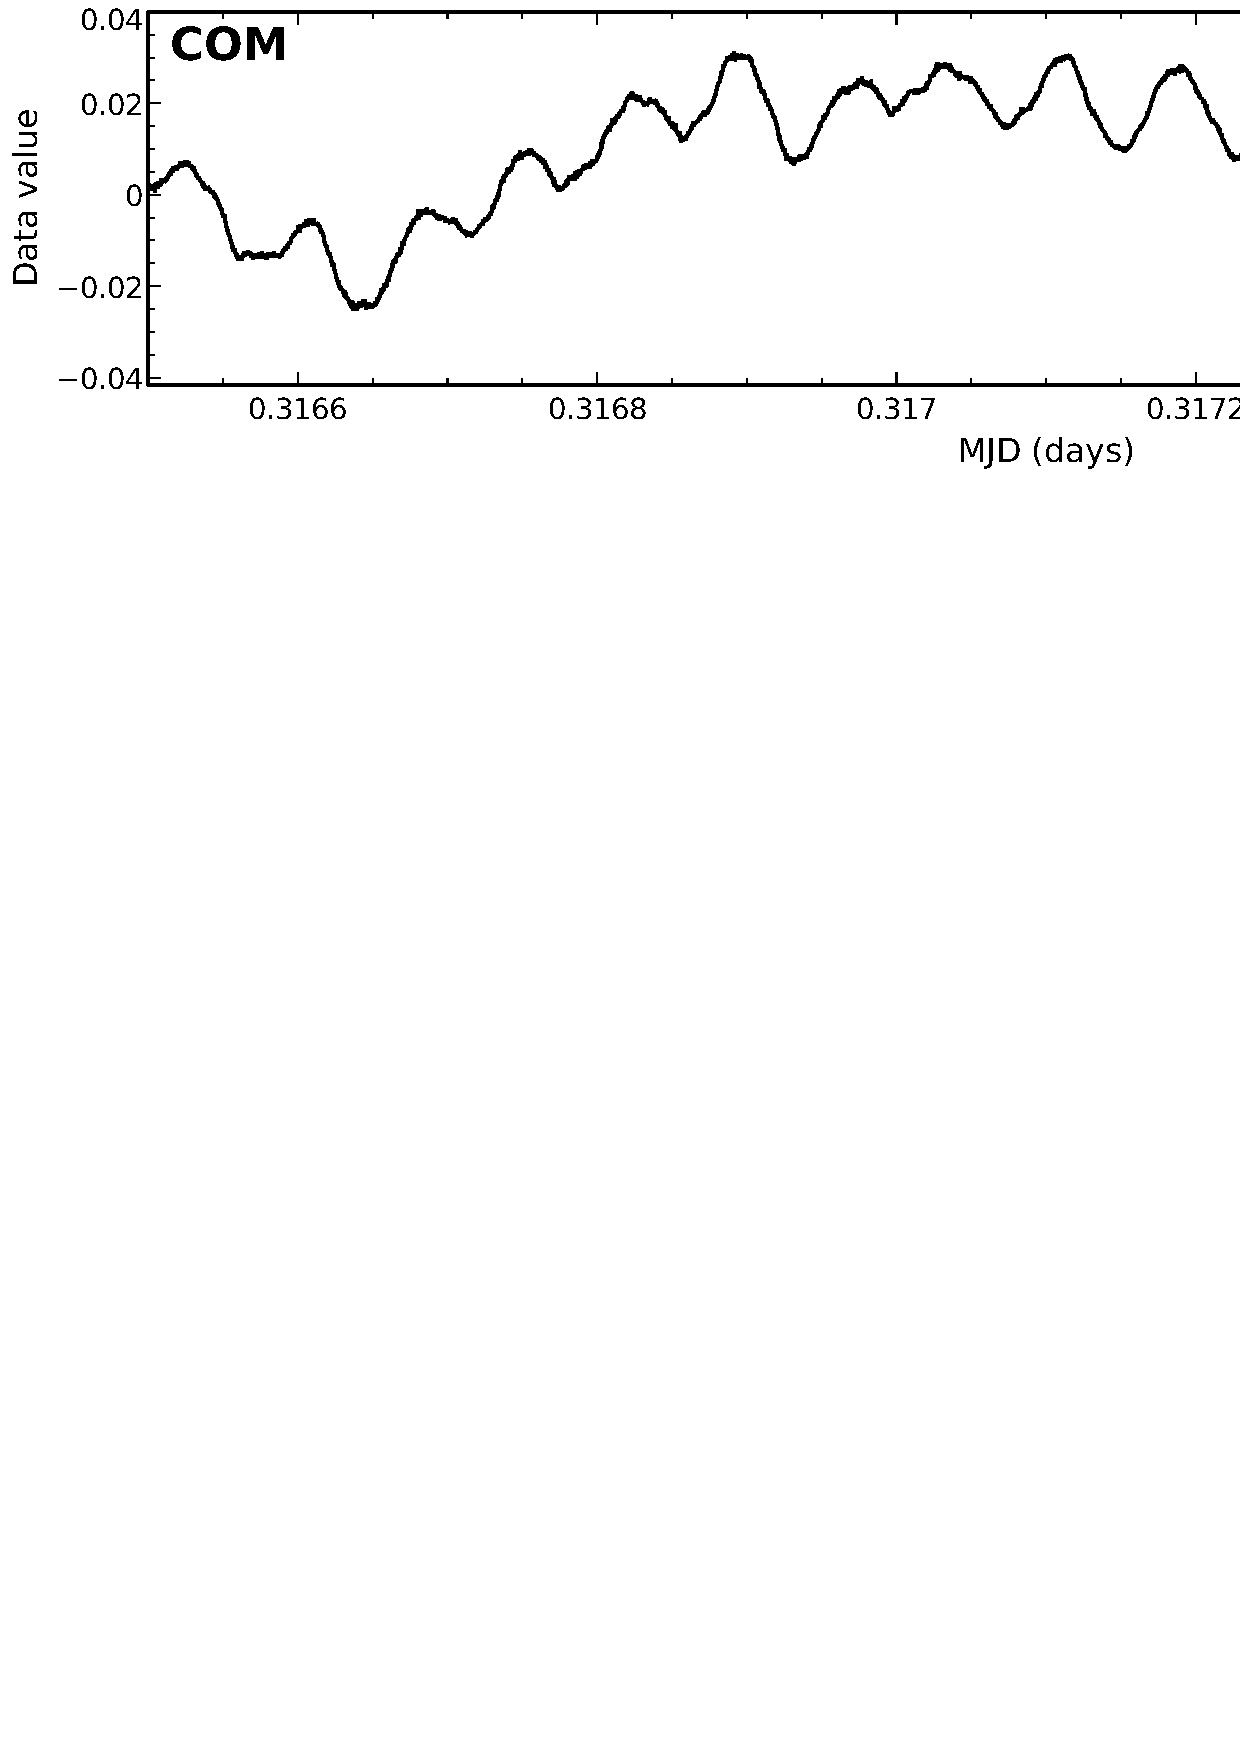
\includegraphics[width=\linewidth]{sc21_com} \\
  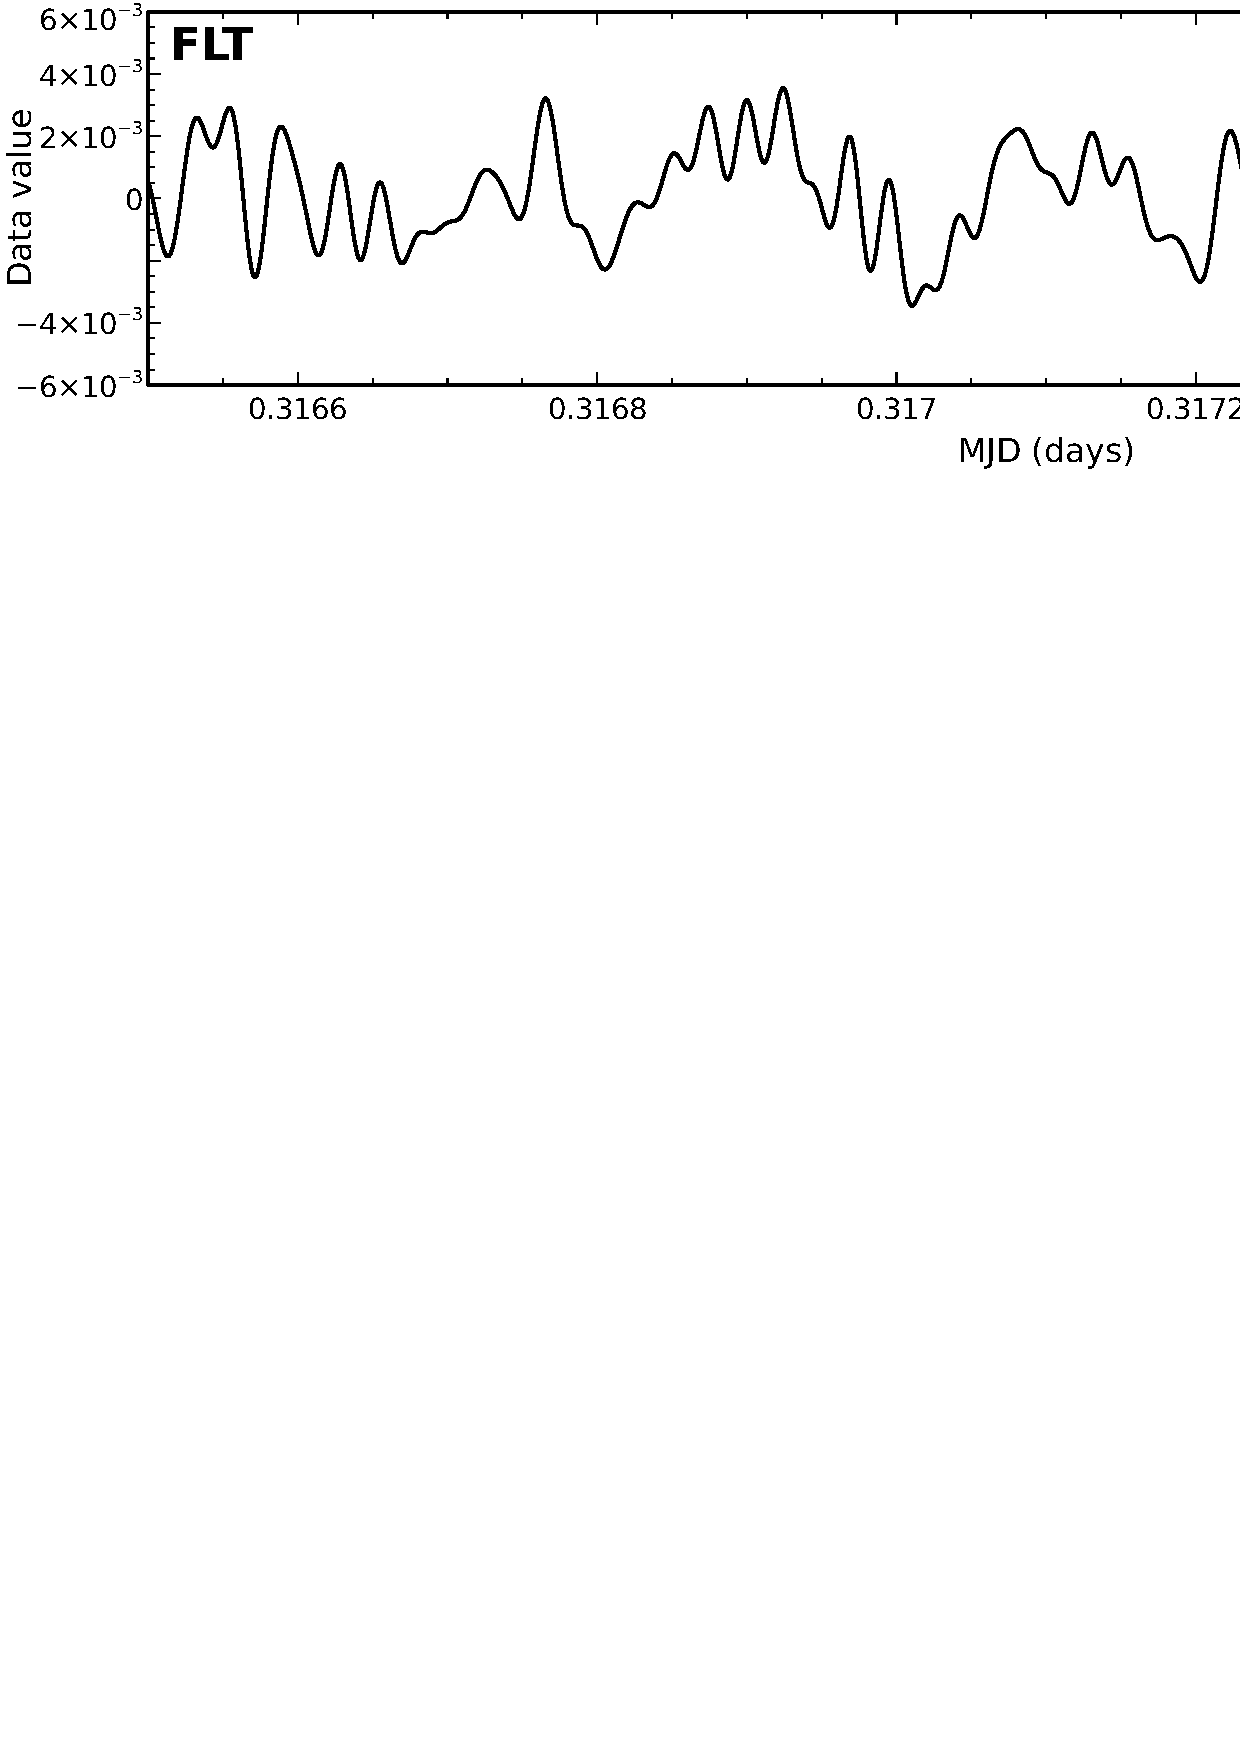
\includegraphics[width=\linewidth]{sc21_flt} \\
  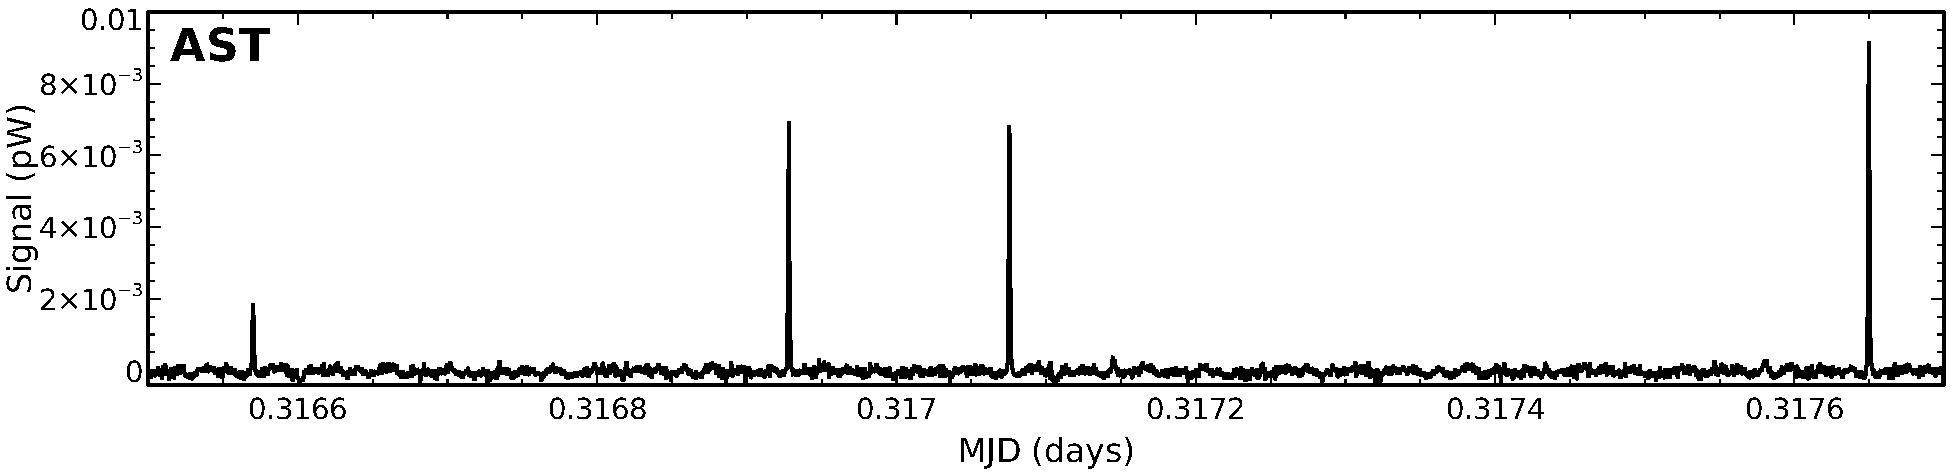
\includegraphics[width=\linewidth]{sc21_ast} \\
  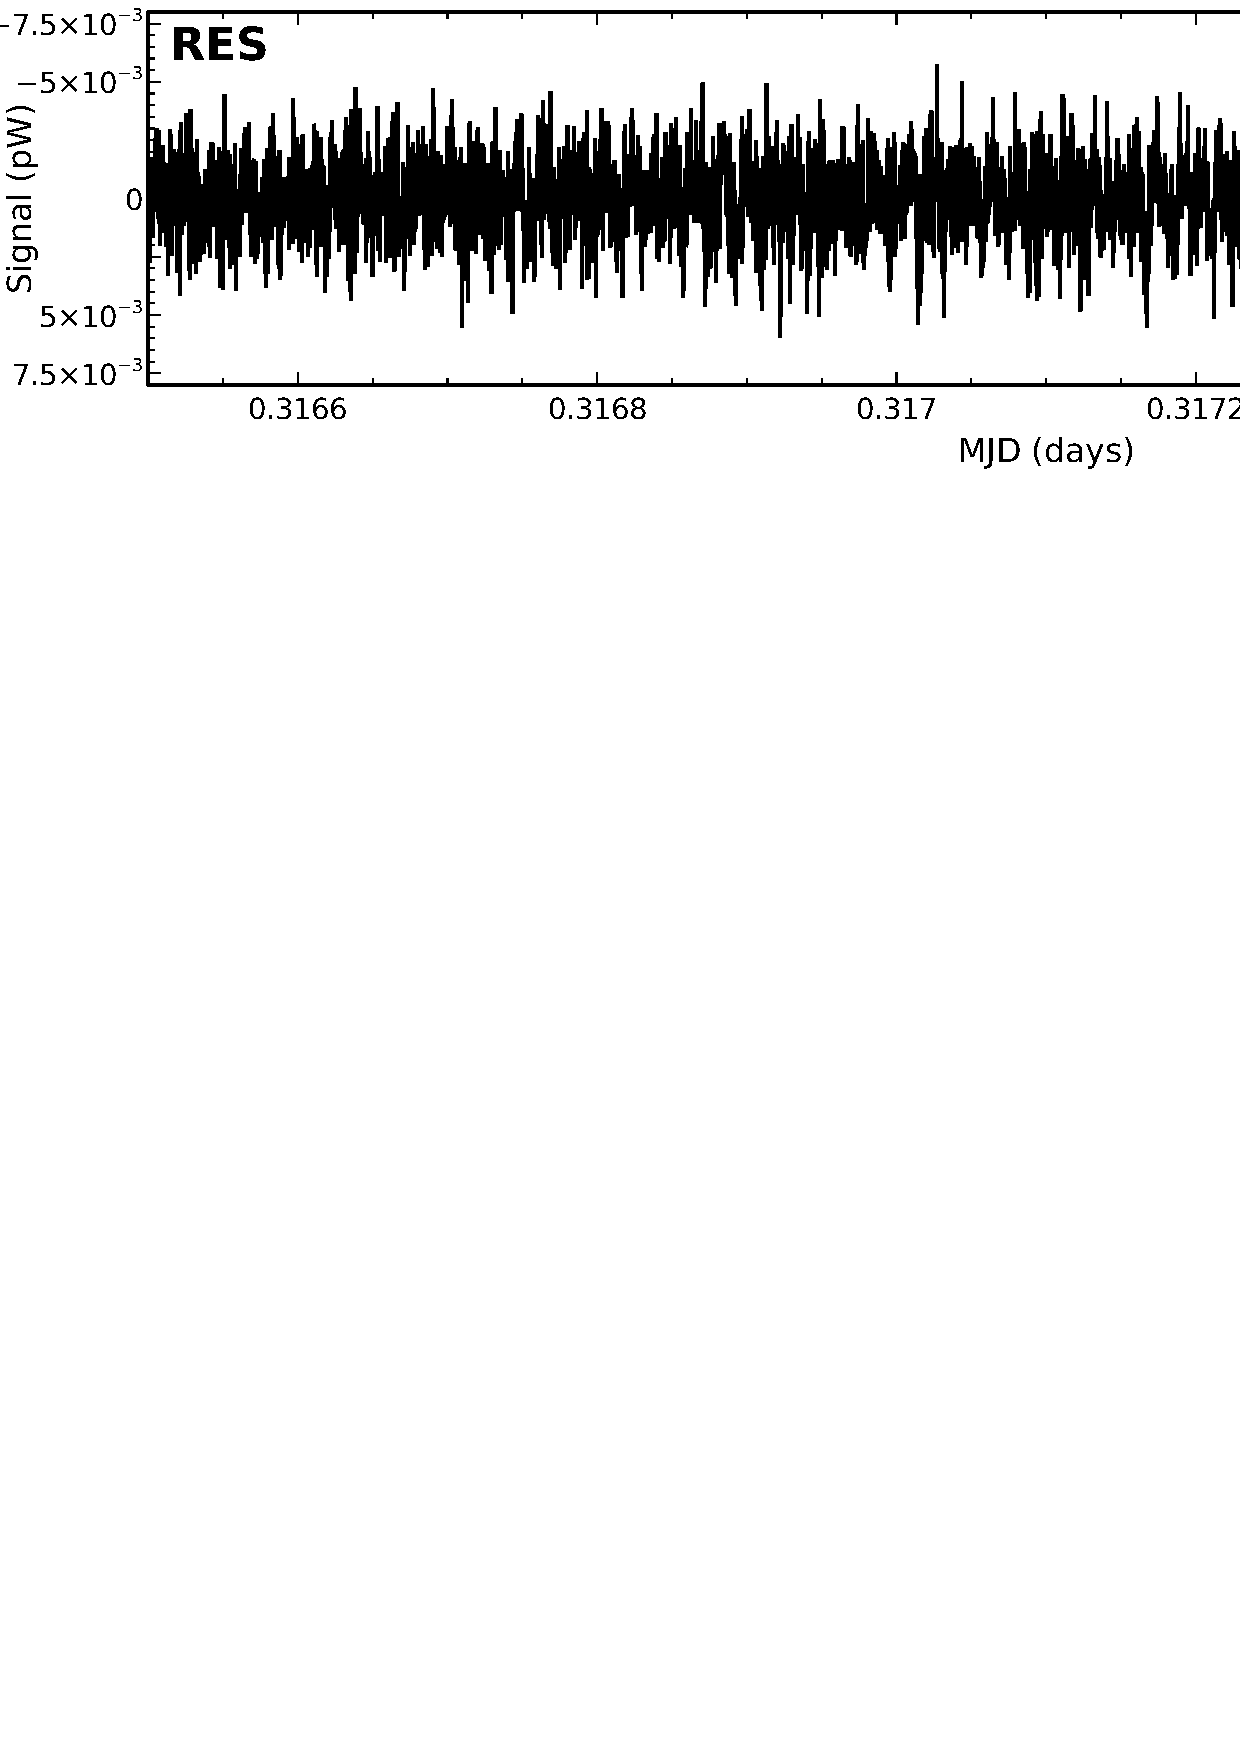
\includegraphics[width=\linewidth]{sc21_res} \\
\end{center}
\caption[Iterative models in the time domain]{\small Time-domain
components of the iterative models. These show the solution for the
same single bolometer for part of an observation of CRL~2688. From top
to bottom: the \model{COM} model containing signal common to all
bolometers, the \model{FLT} model containing residual low-frequency
noise missed by \model{COM}, the \model{AST} model with the signal
showing as a positive spike when this bolometer passes over the
source, and the \model{RES} model looking (as expected) like white
noise.}
\label{fig:itercomp}
\end{figure}


\section{\xlabel{export}Exporting individual models}
\label{sec:export}

By default, the final values of these fitted models are \emph{not}
written out. However, this can be changed by setting
\xparam{EXPORTNDF}{exportndf} in the configuration file to the list of models
that you wish to view.
%\vspace{0cm}

\begin{terminalv}
exportndf = (com,gai,ast,flt,res,noi,qua)
\end{terminalv}

In addition to the models listed in \cref{Section}{sec:models}{The
individual models}, you request \model{RES} in order to export the
residual model. \model{RES} is the residual signal remaining after
the other models have been removed. By contrast, the \model{NOI}
model is the noise in \model{RES}, as determined by running
\model{RES} through \calcnoise\ (see
\cref{Section}{sec:calcnoise}{Checking the array performance}). If
\model{NOI} is exported, it can be viewed as the VARIANCE component
of the \model{RES} model; thus, export of \model{RES} is implied if
\model{NOI} is specified.


The \texttt{exportndf} parameter will write out the requested models
as NDF files with names based on the first input file that went into
the maps for each sub-array. This is first suffixed by \texttt{con},
indicating that several data files may have been concatenated
together. The three-letter code for each model is then appended to the
filename (such as \file{s8a20120720\_00030\_0003\_con\_com.sdf},
\file{s8a20120720\_00030\_0003\_con\_flt.sdf},
\file{s8a20120720\_00030\_0003\_con\_res.sdf})\footnote{The filename
shows the third sub-scan of Observation 30 since this is the first science
file that is encountered (see \cref{Chapter}{sec:raw}{Handling Raw
SCUBA-2 Data}).~} The variance and quality for the data are stored as
the VARIANCE and QUALITY components within the residual file NDF.

\begin{tip}
  You can examine any of these model components as you would the final
  map.
\end{tip}

Examples of the time traces for a single bolometer from these output
models is shown in \cref{Figure}{fig:itercomp}{time-domain
components}. These traces cover a subset of an observation of the
secondary calibrator CRL~2688. You can clearly see the dominance of the
\model{COM} model which is removed first. The \model{FLT} model
stores the data removed by the high-pass filter. In the \model{AST}
model, CRL~2688 is clearly seen as positive spikes which appear when
the bolometer passes over the source. Finally, the residual signal
stored in \model{RES} is flat, indicating that most of the signal has
been successfully accounted for by the other model components.


\section{\xlabel{config}Specialised configuration files}
\label{sec:config}

Currently all data reduced by the JCMT amd made public through the JCMT Science
Archive are reduced with \file{dimmconfig\_jsa\_generic.lis}. If
If unspecified an observation reduced with the pipeline using REDUCE\_SCAN
This configuration file is intended to provide a reasonably good map
for all types of observations. However, compromises have been made to reach
that balance.

Whilst \file{dimmconfig\_jsa\_generic.lis} is always a good recipe to start with
you will want to follow this up with a specialised recipe that will suit
your observation. A few specialised configuration files are supplied with
\smurf\ and can be found in \file{\$STARLINK\_DIR/share/smurf/}.

The specialised files are all built off a base configuration file called
\file{dimmconfig.lis}. This base file is common to all specialised configuration files.
This common base file is illustrated by \cref{Figure}{fig:configtree}{figure below} where
the parameters in \file{dimmconfig\_bright\_compact.lis} override
any identical ones in the hidden file \file{dimmconfig\_bright.lis} which in turn
override the values in \file{dimmconfig.lis}. The hierarchical
structure means the parameters at the top of the tree (or first
encountered) override any other instance of them.

\starfig{sc21_dimmcongitree}{[t]}{width=\linewidth}{fig:configtree}{
  Hierarchy of the configuration files}{
  Hierarchy of the configuration files.
}

Below is a description of each of the specialised configuration files.
The tables following each description list the parameters set for each
recipe. A verbatim copy of these files can be found in
\cref{Appendix}{app:special}{Specialised configuration files}.

\subsection{dimmconfig\_jsa\_generic.lis}

This configuration is designed to handle all science data. This is a good
configuration file to start if you are unsure how to proceed with your
data reduction. This file also utilises the base configuration file \file{dimmconfig.lis}.

You may notice that elements of this
configuration are common to the other specialised configuration files.

Iteratively applying a high-pass filter (\model{FLT}) can result in
convergence problems when there is little or no signal in the
map. Instead, a single, harsher high-pass filter is applied as a
pre-processing step (corresponding to 200-arcsec scales at both
450\,$\mu$m and 850\,$\mu$m).

\xparam{COM.PERARRAY}{com.perarray} is set to 1 indicating that a \model{COM} model
should be fit separately for each sub-array. This is not ideal for extended structure
but can prevent issues from arising from variations in the common mode.
In addition the S/N threshold for DC steps (\xparam{DCTHRESH}{dcthresh}) is relaxed from
25 in the default file to 100 to avoid problems associated with bright sources.


\latex{\renewcommand*\arraystretch{1}}
\begin{table}[h!]
\centering
\begin{tabular}{|p{6.5cm}p{6.5cm}|}
\hline
\multicolumn{2}{|l|}{\file{dimmconfig\_jsa\_generic.lis}}\\
\hline
\param{numiter~=~-25}&\param{flt.filt\_edge\_largescale~=~200}\\
\param{ast.zero\_snr~=~5}&\param{ast.zero\_snrlo~=~3}\\
\param{ast.skip~=~5}&\param{flt.zero\_snr~=~5}\\
\param{flt.zero\_snrlo~=~3}& \param{maptol~=~0.01}\\
\param{maptol\_mean~=~1}&\param{noi.box\_type~=~1}\\
\param{noisecliphigh~=~10.0}&\param{dcthresh~=~100}\\
\param{com.perarray~=~1}&\\
\hline
\end{tabular}
\end{table}




\subsection{dimmconfig\_blank\_field.lis}

This configuration is tuned for blank field surveys for which the goal
is to detect extremely low signal-to-noise point sources.

Iteratively applying a high-pass filter (\model{FLT}) can result in
convergence problems when there is little or no signal in the
map. Instead, a single, harsher high-pass filter is applied as a
pre-processing step (corresponding to 200-arcsec scales at both
450\,$\mu$m and 850\,$\mu$m). There are also more conservative cuts to
remove noisy/problematic bolometers. Only 4 (positive) iterations are
requested as there is no signal to confuse to models.

The option \xparam{COM.PERARRAY}{com.perarray}~=~1 requires the \model{COM} model to
be fit to each sub-array independently. This improves the overall fit
but with the loss of any structure on scales larger than a single
sub-array---not an issue for blank fields.

\cref{Figure}{fig:bfcompare}{The images below} shows the sharp
contrast in the output map between reducing data with the default
configuration file and using \file{dimmconfig\_blank\_field.lis}.

Blank-field maps commonly have a matched filter applied to aid source
detection (see \cref{Section}{sec:mf}{Point-source detection}),
however this is not applied by the map-maker.

\begin{figure}[t!]
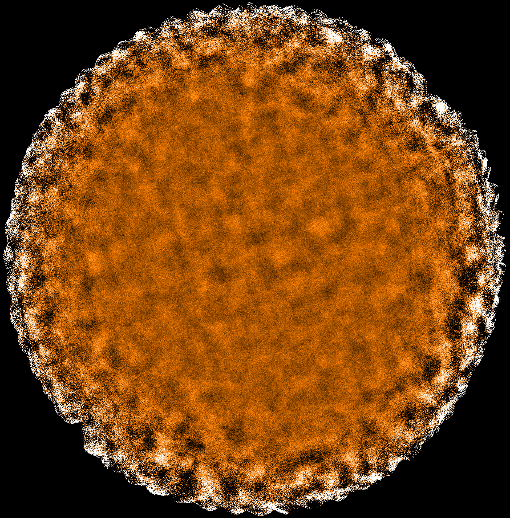
\includegraphics[width=0.47\linewidth]{sc21_cosmo1-def}
\hspace{3mm}
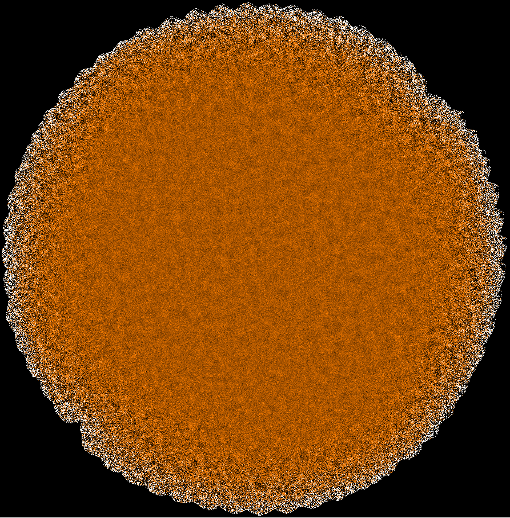
\includegraphics[width=0.47\linewidth]{sc21_cosmo1-bf}
\caption[Example map reduced with \file{dimmconfig\_blank\_field.lis}]{
    Maps of a deep cosmology field reduced with \textbf{(left)}
    \file{dimmconfig.lis} and \textbf{(right)}
    \file{dimmconfig\_blank\_field.lis} \label{fig:bfcompare}}.
\end{figure}



% The tildes around the equal sign are to ensure HTML table field is
% not wrapped after the parameter name.
\renewcommand*\arraystretch{0.95}
\begin{table}[h!]
\centering
\begin{tabular}{|p{6.5cm}p{7.0cm}|}
\hline
\multicolumn{2}{|l|}{\file{dimmconfig\_blank\_field.lis}}\\
\hline
\param{numiter~=~4}&\param{flt\_edge\_largescale~=~200}\\
\param{spikethresh~=~10}&\param{model order~=~(com,ext,ast,noi)}\\
\param{com.perarray~=~1}&\\
\hline
\end{tabular}
\end{table}




\subsection{dimmconfig\_bright\_compact.lis}

This configuration is aimed at reducing maps of bright, compact
sources that are isolated at the centre of the map (i.e. calibrators). It references
\file{dimmconfig\_bright.lis}, and thus the parameters from both `bright'
recipes override the default values in \file{dimmconfig.lis}.

The addition of the \xparam{AST.ZERO_CIRCLE}{ast.zero\_circle} parameter
is used to constrain the map to zero beyond a radius of 1\,arcmin. This
strategy helps with map convergence significantly, and can provide good
maps of bright sources, even in cases where scan patterns failed to
complete in full.

\xparam{COM.PERARRAY}{com.perarray} is set to 1 indicating that a \model{COM} model
should be fit separately for each sub-array. This is not advised for
extended sources as signal on scales larger than a single sub-array is
lost, but is fine for a compact central source. Likewise, the filtering
is tighter. The S/N threshold for DC steps (\xparam{DCTHRESH}{dcthresh}) is relaxed from
25 in the default file to 100 to avoid problems associated with bright sources.

% The tildes around the equal sign are to ensure HTML table field is
% not wrapped after the parameter name.
\latex{\renewcommand*\arraystretch{0.95}}
\begin{table}[h!]
\centering
\begin{tabular}{|p{6.5cm}p{7.0cm}|}
\hline
\multicolumn{2}{|l|}{\file{dimmconfig\_bright\_compact.lis}}\\
\hline
\param{numiter = -40}&\param{flt.filt\_edge\_largescale~=~200}\\
\param{com.perarray~=~1}&\param{flt.zero\_circle~=~(0.016666)}\\
 \param{ast.zero\_circle~=~(0.0166666666)}&\\
\hline
\multicolumn{2}{|l|}{\param{dimmconfig\_bright.lis}}\\
\hline
\param{noisecliphigh~=~10.0} & \param{dcthresh~=~100}\\
\param{com.corr\_tol~=~7}& \param{com.gain\_tol~=~7}\\
\param{com.gain\_abstol~=~5}& \\
\hline
\end{tabular}
\end{table}


\subsection{dimmconfig\_bright\_extended.lis}

\begin{figure}[t!]
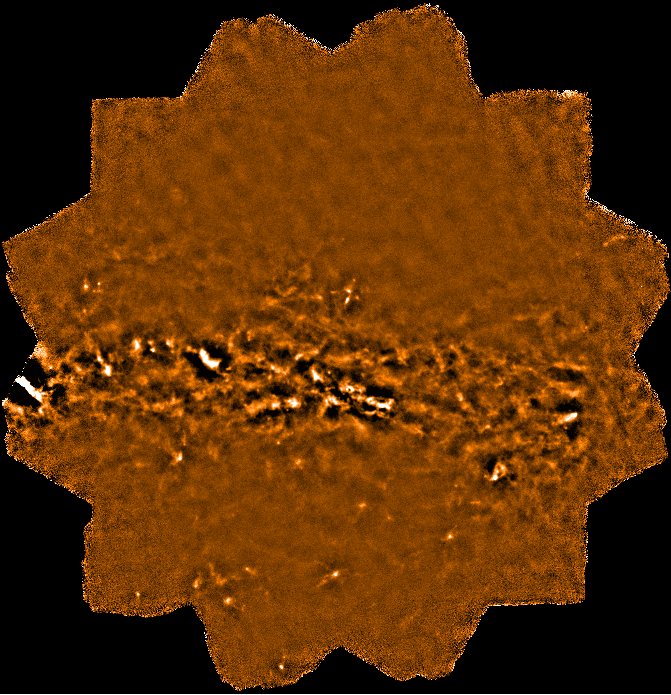
\includegraphics[width=0.47\linewidth]{sc21_gal_def}
\hspace{3mm}
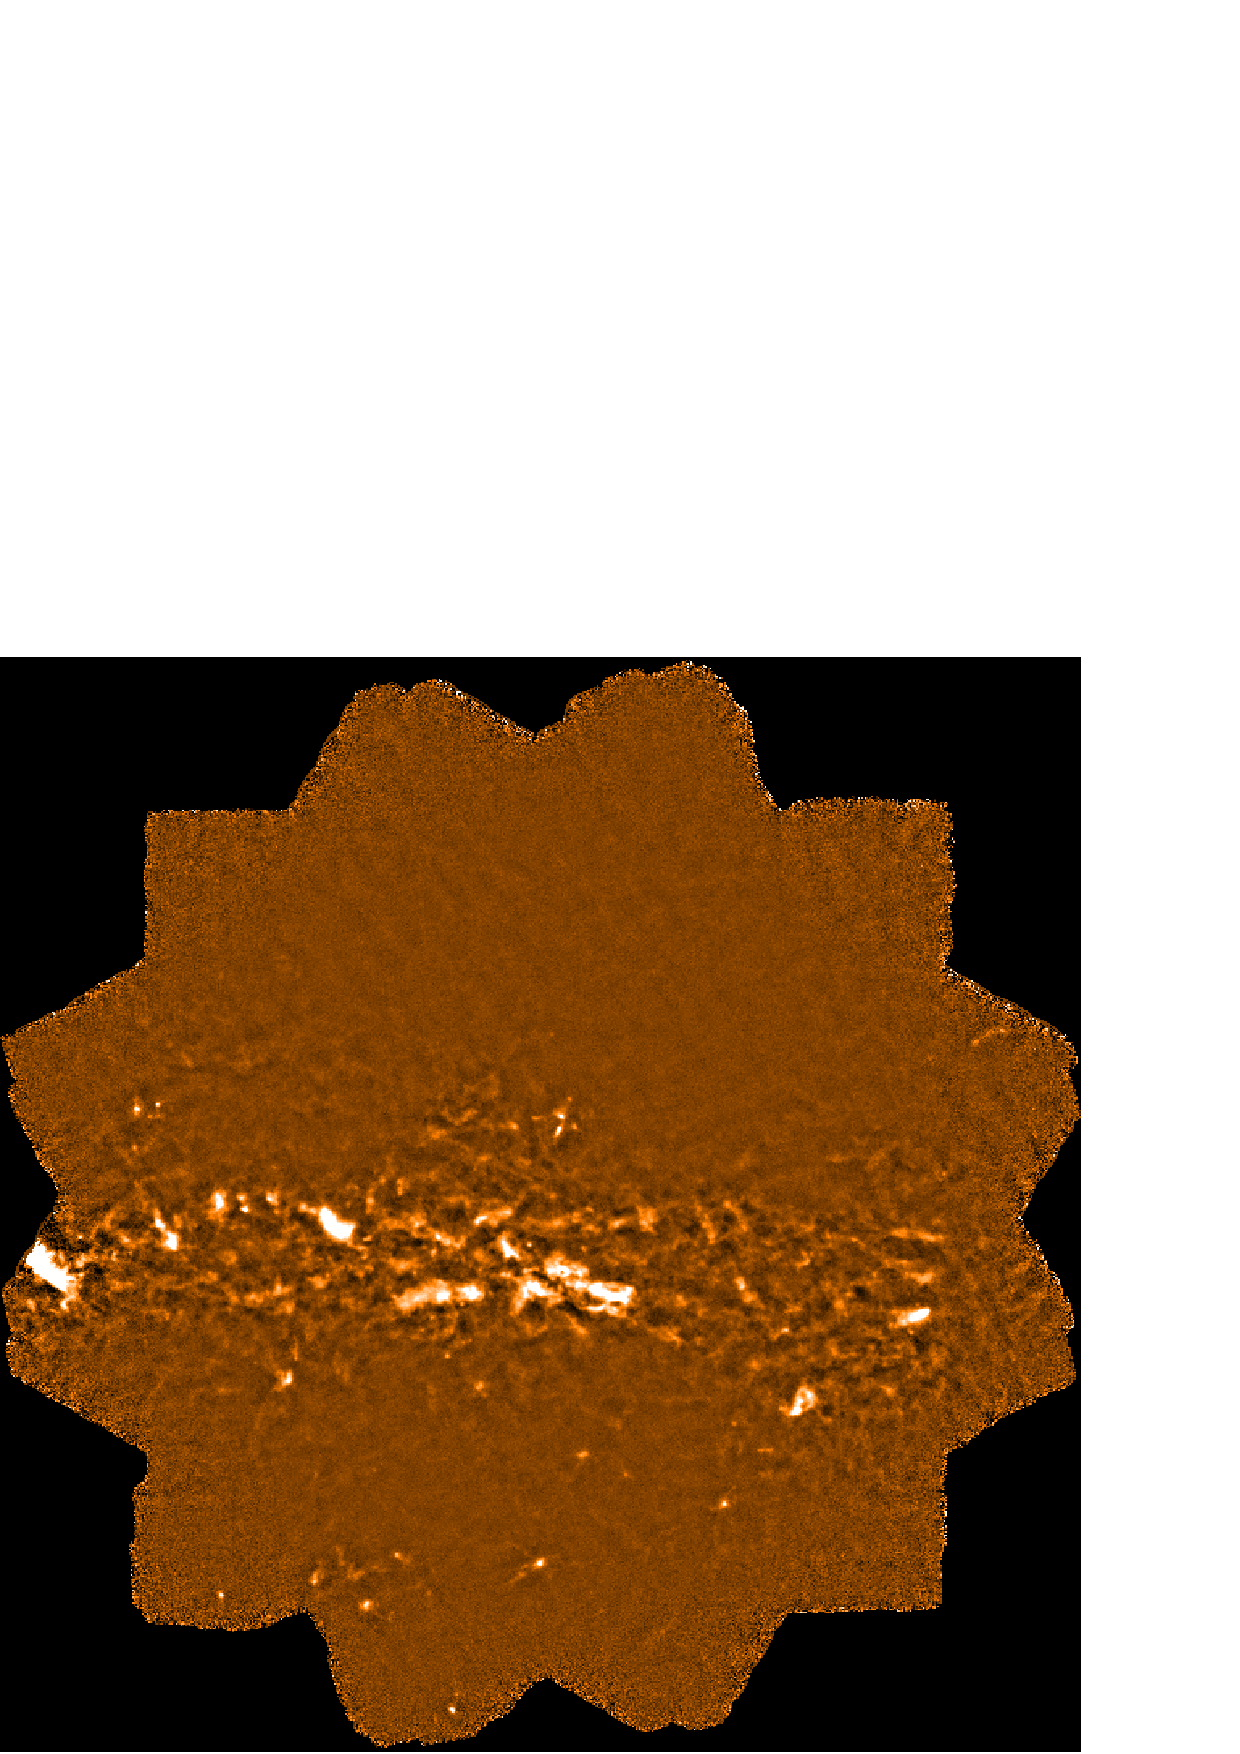
\includegraphics[width=0.47\linewidth]{sc21_gal_brex}
\caption[Example map reduced with
  \file{dimmconfig\_bright\_extended.lis}]
 {A region towards the Galactic Centre reduced with \textbf{(left)}
   \file{dimmconfig.lis} and \textbf{(right)}
   \file{dimmconfig\_bright\_extended.lis}.\label{fig:becompare}}
\end{figure}

This configuration is for reducing maps that do not fall into the
other two categories. The emission is usually extended to some degree
and contains some bright regions. Here \xparam{AST.ZERO_SNR}{ast.zero\_snr} is used
to constrain the \model{AST} model to zero wherever the S/N is lower
than 5$\sigma$.  Everywhere the signal is below this threshold, the
map is set to zero for all but the final iteration. \xparam{NUMITER}{numiter}
has been raised to \texttt{-40}, as more iterations are required to
maximise the sensitivity to large dynamic signal ranges in the map.

Recovering both faint extended structure and bright sources in the
same field poses an extra challenge. Strategies for this are explored
in \cref{Chapter}{sec:tweak}{Tailoring Your Reduction}.

\cref{Figure}{fig:becompare}{The images below} shows a comparison
between maps reduced with the default configuration file and using
\file{dimmconfig\_bright\_extended.lis}; the most noticeable
difference is the improvement in the bowling around strong sources.

\latex{\renewcommand*\arraystretch{1}}
\begin{table}[h!]
\centering
\begin{tabular}{|p{6.5cm}p{6.5cm}|}
\hline
\multicolumn{2}{|l|}{\file{dimmconfig\_bright\_extended.lis}}\\
\hline
\param{numiter~=~-40}&\param{flt.filt\_edge\_largescale~=~480}\\
\param{ast.zero\_snr~=~3}&\param{ast.zero\_snrlo~=~2}\\
\param{ast.skip~=~5}&\param{flt.zero\_snr~=~5}\\
\param{flt.zero\_snrlo~=~3}& \\
\hline
\end{tabular}
\end{table}


\section{\xlabel{problem}Solving configuration-file problems}
\label{sec:problem}

Two trouble-shooting configuration files are available to supplement your
configuration file.
\begin{itemize}[noitemsep]
\item \file{dimmconfig\_fix\_convergence} to help your map converge.
\item \file{dimmconfig\_fix\_blobs} to remove large blooms or blobs of spurious
emission in your map.
\end{itemize}
By default these recipes do not point to any existing configuration file. To use
these recipes in addition to  \file{dimmconfig\_bright\_extended.lis} you should
create a parameter file containing the following lines.

\begin{terminalv}
^/star/share/smurf/dimmconfig_bright_extended.lis
^/star/share/smurf/dimmconfig_fix_blobs.lis
\end{terminalv}

This reads a complete set of configuration parameter from the
\file{dimmconfig\_bright\_extended.lis} file, and then assigns new values for just
those parameters defined in \file{dimmconfig\_fix\_blobs.lis}. These values override
the values specified in \file{dimmconfig\_bright\_extended.lis}.

The parameters in these recipes are discussed further
\cref{Chapter}{sec:tweak}{Tailoring Your Reduction}.




\section{\xlabel{running_dimm}Manually running the iterative map-maker}
\label{sec:running}

The next chapter describes how to run \cref{Chapter}{sec:pipe}{the SCUBA-2 Pipeline}.
Users - particularly new users - are encourage to make use of the \oracdr\ pipeline.
However, greater control of the map-making process is available by running the \makemap\
command directly, rather than from within the pipeline. This section describes how
to do this, but should be seen as ``advanced usage''.

When running the map-maker, you can call any of the provided
configuration files directly from the Starlink path (e.g.
\file{\^{}\$STARLINK\_DIR/share/smurf/dimmconfig.lis}). Alternatively,
a local copy can be made and edited. Advice on which parameters to
edit can be found in \cref{Section}{sec:tweak}{Tweaking the
configuration file}.

\begin{tip}
  An up-caret (\,\texttt{\^{}}\,) is required any time you are reading
  in a group text file in \starlink. For the map-maker this includes
  the configuration file (a group of parameters) and a list of your
  input files (e.g. \texttt{in=\^{}\,myrawfiles.txt}).
\end{tip}


The default pixel sizes are:
\begin{itemize}
\item 2\,arcsec at 450$\mu$m
\item 4\,arcsec at 850$\mu$m
\end{itemize}

These can be changed by adding the \texttt{pixsize=}$x$ to the
command string\footnote{The default sizes are defined as one quarter
of the Airy disk rounded up to the nearest half arcsecond.}, where $x$
is your desired pixel size in arcsecs. We advise that you do not
increase the pixel size at this stage as it will compromise model
fitting---instead regrid your map as a post-processing step.

% Other ADAM parameter available with \makemap\ include ref, maxmem
% and msg\_filter. Some of these appear in the example below but see
% \cref{Appendix}{app:adam}{MAKEMAP ADAM Parameters} for
% descriptions. A complete list of all ADAM parameters can be found in
% \smurfsun.

\begin{tip}
  Map-maker not finding your raw files from a path? Check you have
  double quotes around your `in' option and are not using
  \texttt{*sdf}---use either \texttt{*.sdf} or just \texttt{*}.
\end{tip}



\begin{terminalv}
% makemap in="/jcmtdata/raw/scuba2/s8*/20120720/00030/*.sdf" out=850_crl2688 \
  config=^$STARLINK_DIR/share/smurf/dimmconfig.lis

Out of 32 input files, 4 were darks, 8 were fast flats and 20 were science
Processing data from instrument 'SCUBA-2' for object 'CRL2688' from the
following observation  :
  20120720 #30 scan  /shutter

MAKEMAP: Map-maker will use no more than 68401 MiB of memory

Projection parameters used:
CRPIX1 = 0
CRPIX2 = 0
CRVAL1 = 315.578333333333 ( RA = 21:02:18.800 )
CRVAL2 = 36.6938055555556 ( Dec = 36:41:37.70 )
CDELT1 = -0.00111111111111111 ( -4 arcsec )
CDELT2 = 0.00111111111111111 ( 4 arcsec )
CROTA2 = 0

Output map pixel bounds: ( -132:122, -126:129 )

Output map WCS bounds:
Right ascension: 21:01:38.318 -> 21:03:03.280
Declination: 36:33:07.19 -> 36:50:11.70

smf_iteratemap: will down-sample data to match angular scale of 4 arcsec
smf_iteratemap: Iterate to convergence (max 5)
smf_iteratemap: stop when change in chi^2 < 0.001
smf_iteratemap: provided data are in 1 continuous chunks, the largest of which
has 5957 samples (153.729 s)
smf_iteratemap: map-making requires 1376 MiB (map=3 MiB model calc=1372 MiB)
smf_iteratemap: Continuous chunk 1 / 1 =========
smf_calc_smoothedwvm: 0.977444 s to calculate unsmoothed WVM tau values
smf_iteratemap: Iteration 1 / 5 ---------------
--- Size of the entire data array ------------------------------------------
bolos  : 5120
tslices: bnd:0(0.0 min), map:5957(2.6 min), tot:5957(2.6 min)
Total samples: 30499840
--- Quality flagging statistics --------------------------------------------
 BADDA:   10972794 (35.98%),        1842 bolos
BADBOL:   11818688 (38.75%),        1984 bolos
DCJUMP:      38809 ( 0.13%),
  STAT:      71680 ( 0.24%),          14 tslices
 NOISE:     810152 ( 2.66%),         136 bolos
Total samples available for map:   18634826, 61.10% of max (3128.22 bolos)
smf_iteratemap: Calculate time-stream model components
smf_iteratemap: Rebin residual to estimate MAP
smf_iteratemap: Calculate ast
--- Quality flagging statistics --------------------------------------------
 BADDA:   10972794 (35.98%),        1842 bolos  ,change          0 (+0.00%)
BADBOL:   11925914 (39.10%),        2002 bolos  ,change     107226 (+0.91%)
DCJUMP:      38809 ( 0.13%),                    ,change          0 (+0.00%)
  STAT:      71680 ( 0.24%),          14 tslices,change          0 (+0.00%)
   COM:     323165 ( 1.06%),                    ,change     323165 (+0.00%)
 NOISE:     810152 ( 2.66%),         136 bolos  ,change          0 (+0.00%)
Total samples available for map:   18312771, 60.04% of max (3074.16 bolos)
     Change from last report:    -322055, -1.73% of previous
smf_iteratemap: Will calculate chi^2 next iteration
smf_iteratemap: *** NORMALIZED MAP CHANGE: 0.874979 (mean) 73.7106 (max)
smf_iteratemap: Iteration 2 / 5 ---------------
smf_iteratemap: Calculate time-stream model components
smf_iteratemap: Rebin residual to estimate MAP
smf_iteratemap: Calculate ast
--- Quality flagging statistics --------------------------------------------
 BADDA:   10972794 (35.98%),        1842 bolos  ,change          0 (+0.00%)
BADBOL:   11949742 (39.18%),        2006 bolos  ,change      23828 (+0.20%)
 SPIKE:         34 ( 0.00%),                    ,change         34 (+0.00%)
DCJUMP:      38809 ( 0.13%),                    ,change          0 (+0.00%)
  STAT:      71680 ( 0.24%),          14 tslices,change          0 (+0.00%)
   COM:     357816 ( 1.17%),                    ,change      34651 (+10.72%)
 NOISE:     810152 ( 2.66%),         136 bolos  ,change          0 (+0.00%)
Total samples available for map:   18278374, 59.93% of max (3068.39 bolos)
     Change from last report:     -34397, -0.19% of previous
smf_iteratemap: *** CHISQUARED = 0.983228126551834
smf_iteratemap: *** NORMALIZED MAP CHANGE: 1.29181 (mean) 15.0552 (max)
smf_iteratemap: Iteration 3 / 5 ---------------
.....
.....
.....
smf_iteratemap: Iteration 5 / 5 ---------------
smf_iteratemap: Calculate time-stream model components
smf_iteratemap: Rebin residual to estimate MAP
smf_iteratemap: Calculate ast
--- Quality flagging statistics --------------------------------------------
 BADDA:   10972794 (35.98%),        1842 bolos  ,change          0 (+0.00%)
BADBOL:   11949742 (39.18%),        2006 bolos  ,change          0 (+0.00%)
 SPIKE:         34 ( 0.00%),                    ,change          0 (+0.00%)
DCJUMP:      38809 ( 0.13%),                    ,change          0 (+0.00%)
  STAT:      71680 ( 0.24%),          14 tslices,change          0 (+0.00%)
   COM:     362902 ( 1.19%),                    ,change          0 (+0.00%)
 NOISE:     810152 ( 2.66%),         136 bolos  ,change          0 (+0.00%)
Total samples available for map:   18273302, 59.91% of max (3067.53 bolos)
     Change from last report:          0, +0.00% of previous
smf_iteratemap: *** CHISQUARED = 0.952708604771402
smf_iteratemap: *** change: -0.000109049487216351
smf_iteratemap: *** NORMALIZED MAP CHANGE: 0.107427 (mean) 2.96138 (max)
smf_iteratemap: ****** Completed in 5 iterations
smf_iteratemap: ****** Solution CONVERGED
Total samples available from all chunks: 18273302 (3067.53 bolos)
%%%%\end{}
\end{terminalv}




